\graphicspath{{chapt_dutch/}{intro/}{chapt2/}{chapt3/}{chapt4/}{chapt5/}{chapt6/}{chapt7/}{chapt8/}}

% Header
\renewcommand\evenpagerightmark{{\scshape\small Chapter 4}}
\renewcommand\oddpageleftmark{{\scshape\small Signal Generation and Simulation}}

\renewcommand{\bibname}{References}

\hyphenation{}

\chapter[Signal Generation and Simulation]%
{Signal Generation and Simulation}\label{chapt:4}
\section{Monte Carlo simulation}\label{sec:mc_sim}
In high energy physics experiments, event modelling plays an important role to understand the collected data. A precisely modelled event maximizes the chance to find out new physics and make precision measurement of the Standard Model processes. However, in hadron-hadron colliders where the colliding particles are composite objects, like proton-proton in LHC, the event modelling is a challenging task. The same applies to particles interactions within the bulk of detector volume. These tasks can be solved by employing Monte Carlo generation techniques, incorporating the Standard Model, models of new physics and the detector effects while detecting final state particles in the interaction. An event occurs when two protons collide and produces a cascade of new particles as shown in figure \ref{fig:event}. Because of complexity of the event, the MC generators model the events in a simulation chain: hard interaction, parton showering, hadronization and decays. These processes are explained in the following sections.
\begin{figure}[h]
\centering
%\captionsetup{width=0.8\linewidth}
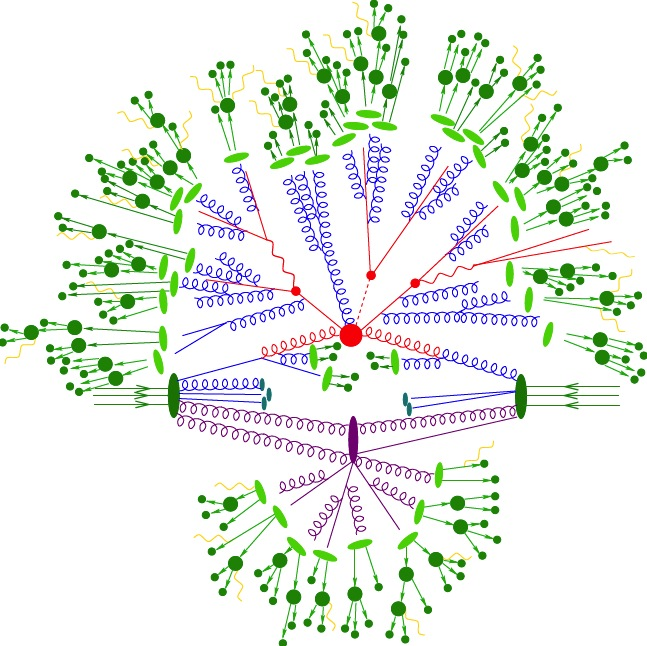
\includegraphics[width=0.6\textwidth]{fig/chapt4/event_sim.jpeg}
%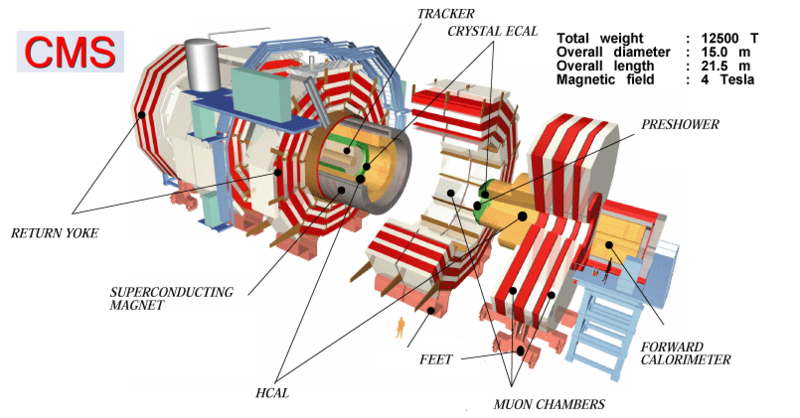
\includegraphics[scale=0.4, trim=20 50 60 30,clip]{fig/chapt3/CMS_exper.png}
\caption{\label{fig:event}Pictorial representation of a $pp$ collision event \cite{simulated_event}. The hard interaction shown by the big red blob. Additional hard QCD radiation is produced (red) and a secondary interaction takes place (purple blob) before the final-state partons hadronise (light green blobs) and hadrons decay (dark green blobs). Photon radiation occurs at any stage (yellow)}
\end{figure}  
\begin{itemize}
\item{\textbf{Hard scattering:}}
The actual interaction of two protons occurs when partons (constituents of proton - gluons or quarks -) from the two colliding protons interact and produce new particles with high $p_{T}$. These events are of keen interest for analysis and referred as hard scattering. If the colliding protons merely undergo soft collision, resultant particles have low $p_{T}s$, commonly known as soft scattering. The parton distribution functions (PDFs) describing the structure of the proton and contained the initial momentum distribution of the partons involved in the hard interaction. In hadron-hadron (in case of LHC it is $pp$) collisions, a wide variety of hard scattering cross sections can be calculated using the QCD factorization theorem and weighting the subprocess cross section with the PDFs extracted from deep inelastic scattering \cite{hard_scatter}. Factorization theorems separate long- and short-distance physics when calculating these cross sections.   
\begin{equation}\label{eq:xsec}
\sigma_{AB} = \int dx_{a}dx_{b}f_{a/A}(x_{a},\alpha_{s},\mu_{F}).f_{b/B}(x_{b},\alpha_{s},\mu_{F}).\hat{\sigma}(\hat{s};\alpha_{s},\mu_{F},\mu_{R})
\end{equation}  
where $f_{a/A}$ is the the probability that a parton $a$ inside a hadron $A$ carries a momentum fraction $x_{a}$, $\hat{s}$ is the parton center-of-mass energy, $\alpha_{s}$ is the strong coupling constant, $\mu_{F}$ is the factorization and $\mu_{R}$ is the renormalization scale.
\item{\textbf{Parton showering:}}
The previous section illustrates generation of a hard process according to lowest-order matrix elements that results in a limited number of partons in the final state. These describe the momenta of the outgoing jets well, but any fixed order is insufficient to give a complete picture of overall process including the internal structure of the jets and the distributions of accompanying particles. The effect of all higher-order corrections including additional ISR/FSR from the branching of the partons can be simulated through the parton-shower (PS) algorithm. It describes the evolution in momentum transfer down from the high energy scales associated with the hard process to the low scales, of order 1 GeV, associated with confinement of the partons it describes into hadrons \cite{parton_shower}. The multi-purpose event generators like PYTHIA \ref{subsec:pythia} and HERWIG \ref{subsec:herwig} used parton showering algorithms with different implementations. Hard processes can be described well using matrix element calculations where the partons are energetic and widely separated. It also incorporates the interference effects of amplitudes with the same final state topology. In this work we produce the interference effect between the signal ($gg\rightarrow H/A\rightarrow t\bar{t}$) and SM $t\bar{t}$ ($gg\rightarrow t\bar{t}$) background. Matrix element and parton shower algorithms can be combined to fully describe an event with an extra care to avoid double counting in the overlapping phase-space. Different schemes are using for this purpose. CMS uses MLM algorithm for matching to interface MADGRAPH with PYTHIA, which vetoes the emission of partons via showering above a user-defined matching threshold \cite{matching}.  
\item{\textbf{Hadronization:}}
Hadronization process starts after showering by which a set of colored partons is transformed into a set of color-singlet
primary hadrons, may decay further to secondary hadrons. Different models are in use to describe the fragmentation of the
partons after showering. The most commonly used one is the $Lund$ $String$ $Fragmentation$ $Model$, implemented in PYTHIA and proposed to be universal i-e process independent. It is based on the observation that the colour potential of the sources, such as a heavy quark–antiquark pair, increases linearly with their separation like a stretched string has $V(r) = \kappa r$. The potential energy increases with the separation of quark anti-quark and at order of 1 fm, it collapses into colour-field strings between them. The original quark pair are now converted into two pairs of quark and anti-quark $q\bar{q}\rightarrow q\bar{q}^{'} + q^{'}\bar{q}$ while this process continues until only hadrons remain \cite{hadronization}. Apart from the hard interaction, other constituents of the colliding proton can also interact, add additional hadrons in the final state. This is usually referred as underlying event (UE) described by special tunes in the generators like PYTHIA uses $CUETP8M2T4$ in this analysis. During one bunch crossing the average pp interaction goes up to 35, known as pileup, resulting into relatively low $p_{T}$ particles, but they can obscure the interesting hard process.
\end{itemize}
\section{Particle Physics Generators}\label{sec:gnerators}
In current High Energy Physics (HEP) regime, the most challenging part is the multiparticle production where the observed particles multiplicities extend to hundred. These multiplicities are expected to go upward in the future HEP colliders. Event Generators (EG), based on computer programs, solve this problem by generating events as detailed as could be observed by a perfect detector.   
In High Energy Physics (HEP), a number of Monte Carlo (MC) generators are available that calculate the tree-level diagrams numerically, and integrate over the relevant phase space. A list of them are used in monte carlo production for this analysis is discussed below.
\subsection{MadGraph}
MadGraph, now merged into MG\_aMC@NLO, a general-purpose event generator \cite{madgraph}, used for generation of the signal samples in this analysis. It is a pure matrix element generator that generates hadron-hadron ($pp, p\bar{p}, gg, q\bar{q}$) collision and in practice produces 8 particles (quarks, gluons and leptons) in the final state without hadronization. It also provides an opportunity to produce samples using interference effect. The interference comes into play when the signal and background have the same final state particles like in this analysis the signal is $gg\rightarrow H/A \rightarrow t\bar{t}$ and the standard model $t\bar{t}$, the main background, have same final state particles. 
MadGraph is further interfaced with Pythia or Herwig to generate showering and hadroziation steps. The double counting in the showering is solved by applying the MLM scheme. To describe the parton structure, NNPDF30 PDF \cite{pdf_sets} sets used in this analysis. 

\subsection{Pythia}\label{subsec:pythia}
Pythia is a multipurpose event generator used frequently in HEP. It provides the possibility to generate complete events, in as much detail as experimentally observable ones, within the bounds of our current understanding of the underlying physics. Pythia is used to model $e^{+}e^{-}$, $ep$ and $pp$ collisions and simulates a large variety (over 300) of hard 2 $\rightarrow$ 2 processes which include Standard Model and many beyond Standard Model processes upto Leading Order (LO) accuracy. Pythia uses Lund string model \cite{lund_string_model} to describe hadronization and external PDFs for hard processes calculations. It uses $p_{T}$-ordered showering technique for parton showering where partons are ordered by their transverse momentum ($p_{T}$) and $Q^{2} = p^{2}_{T}$ - the closer the parton approaches the vicinity of the hard process, the higher pT is assigned to it. A more detail about the Pythia program is given in \cite{pythia}.
\subsection{Powheg}
The Powheg (PositiveWeight Hardest Emission Generator) event generator \cite{powheg} provides the modeling of the hard interaction and needs to be interfaced with Pythia or Herwig for the parton showering and hadronization. Powheg models the hard process at NLO QCD accuracy. The proton structure is described by the PDF sets NNLOPDF30.
\subsection{MC@NLO}
The MC@NLO \cite{mcanlo} is an event generator which generates hard emission using NLO and MC approaches. For showering and hadronization, the MC@NLO has to be interfaced with general purpose detector like pythia. It also generates a small fraction of events with negative weights but in practice it is quite small. The PDF sets used by MC@NLO are NNPDF30.
\subsection{HERWIG}\label{subsec:herwig}
HERWIG is a general-purpose event generator \cite{herwig} which models hadron-hadron, lepton-lepton and hadron-lepton collisions at LO. Like Pythia, it provides the description of all subprocesses of an event but uses different approaches and algorithms. HERWIG tool implements an angular order showering, $Q^{2} \sim 1 - cos\theta$, where $\theta$ is the angle between parent and emitted parton. HERWIG exploits cluster model for showering.
\subsection{2HDMC and SusHi}\label{subsec:sushi}
\textbf{2HDMC:} Two-Higgs-Doublet Model Calculator \cite{2hdmc} is a general purpose calculator based on C++ code which can be used to study the phenomenology of a general ($\textsl{CP}$-conserving) two-higgs doublet model (2HDM) \ref{subsec:2hdm}. 2HDMC provided a user friendly interface to implement its favourite parameters space for the higgs potential. A user has fully control over the Yukawa sector by changing the coupling. The higgs masses, type of the model (type I and type II), alignment limit condition $sine (\alpha - \beta)$, the ratio of the vacuum expectation values of the doublet in 2HDM ($tan\beta$) and the scalar mass matrix, m$^{2}_{12}$, etcetera, can be specified with full freedom. The output of the 2HDMC consists of a check on the theoretical properties of the model like, $\textsl{CP}$-conservation, positivity and stability of the potential and the tree level unitarity and perturbativity. 2HDMC can be used to calculate the higgs decay widths and branching ratios.\\
This work uses 2HDMC to calculate decay widths of the neutral higgs sector, scalar (H) or pseudo-scalar (A), by making an iteration over the $tan\beta$ values. The signal samples has been generated for heavy higgs (scalar and pseudo-scalar) using madgraph for fixed masses and widths. The considered masses are, 400, 500, 600 and 750 GeV while for each mass five width values (1, 5, 10, 25, 50)\% are taking into account. In the 2HDMC, I use fixed values for charged higgs mass (mC = 600 GeV), scalar or pseudo-scalar higgs mass (mA/H = 400 GeV), sine ($\alpha - \beta$) = 1, $\lambda_{6,7}$ = 0 and $m^{2}_{12} = m^{2}_{A}tan\beta/(1 + tan^{2}\beta)$. An iteration over the tan$\beta$ values has done and selected the one that gives the corresponding width used in madgraph generation. The same procedure has repeated for all masses. The selected $tab\beta$ values further used in the SusHi as input.\\    
\textbf{SusHi:} $\textsc{Supersymmetric Higgs}$ \cite{sushi} is a Fortran based program designed to calculate inclusive Higgs-boson production cross sections upto NNLO QCD through gluon fusion and bottom-quark annihilation in the Standard Model (SM), general Two-Higgs-Doublet Models (2HDM), the Minimal Supersymmetric Standard Model (MSSM) as well as its next-to-minimal extension (NMSSM). The program can also be used to calculate differential cross sections with respect to the Higgs transverse momentum $p_{T}$ and (pseudo-)rapidity y($\eta$). SusHi can be linked with 2HDMC calculator for 2HDM calculation, to FeynHiggs for the the MSSM Higgs masses calculations and many more. In this work SusHi links with 2HDMC for the study of neutral higgs LO and NNLO cross sections calculations in 2HDM/hMSSM and incorporated the PDF effects by using external PDF sets (NNPDF30). The factorization and normalization scales are fixed with respect to the neutral higgs mass ($\mu_{F/R} = m_{A/H}/2$). The output card of the 2HDMC used as input in SusHi with 2HDM model in the physical higgs basis. The $tan\beta$ value that corresponds to a certain width has used as a coupling modifier ($g_{A/H}\rightarrow t\bar{t}$) in the madgraph parameter card. The output of LO cross sections from SusHi is comparable with the madgraph cross sections shown in table \ref{table:mg_sushi_compare}. The k-factor calculated as a ratio of NNLO SusHi cross sections to LO with errors and plotted in figure \ref{fig:k_factor}. The results are interpreted as to weight the SM cross section with these k-factors. 
\begin{landscape}
\begin{table}[ht]
\caption{Comparison of leading order cross section from MadGraph and SusHi for pseudo-scalar resonance with masses 400, 500 and 600 GeV and scalar mass = 700 GeV. The k-factor shows universality for a single mass point which is calculated as the ratio of NNLO from SusHi and MadGraph LO cross sections.}
\centering
\begin{tabular}{| c | c | c | c | c | c | c | c | c | c |}
\hline\hline
Mass (GeV) & Width (GeV) & tan$\beta$ & $\frac{1}{tan\beta}$ & LO $\sigma(MG)$ pb & LO $\sigma(SusHi)$ pb & NNLO $\sigma(SusHi)$ pb & BR (A$\rightarrow t\bar{t}$) & K = $\frac{NNLO \sigma(SusHi)}{\sigma(MG)}$ \\ 
\hline\hline
\multirow {6}{*}{400}& 4.002 & 1.908 &  0.52410901467 & 3.641$\pm$0.003587 &  3.63478$\pm$0.0000 & 7.71736$\pm$0.00795 & 9.880$10^{-01}$ & 2.12$\pm$0.003\\
\cline{2-9}
& 10 & 1.2068 & 0.82863771958 & 9.096$\pm$0.009417 & 9.13195$\pm$0.0 & 19.26195$\pm$0.01987 & 9.950$10^{-01}$ & 2.118$\pm$0.009417\\
\cline{2-9}
& 19.49 & 0.8645 & 1.15673799884 & 17.76$\pm$0.01694 & 17.82577$\pm$0.00001 & 37.51884$\pm$0.03872 & 9.960$10^{-01}$ & 2.113$\pm$0.0030\\
\cline{2-9}
& 38.99 & 0.6113 & 1.63585800752 & 35.47$\pm$0.03629 & 35.68351$\pm$0.00002 & 75.01936$\pm$0.07743 & 9.963$10^{-01}$ & 2.115$\pm$0.0031\\
\cline{2-9}
& 97.52 & 0.3865 & 2.5873221216 & 88.86$\pm$0.07161 & 89.31375$\pm$0.00005 & 187.64029$\pm$0.19371 & 9.963$10^{-01}$ & 2.112$\pm$0.0028\\
\cline{2-9}
& 195 & 0.2733 & 3.65898280278 & 177.3$\pm$0.1163 & 178.65641$\pm$0.00009 & 375.25547$\pm$0.38741 & 9.963$10^{-01}$ & 2.117$\pm$0.0026\\
\hline \hline
\multirow {6}{*}{500} & 5.032 & 2.12 & 0.4716981132 & 0.9349$\pm$0.0007767 & 0.94977$\pm$0.0000 & 1.90812$\pm$0.00263 & 9.627$10^{-01}$ & 2.041$\pm$0.0033\\
\cline{2-9}
&12.4 & 1.3506 & 0.73746312684 & 2.291$\pm$0.002217 & 2.32963$\pm$0.000 & 4.66077$\pm$0.00648 &9.854$10^{-01}$ & 2.034$\pm$0.0034\\
\cline{2-9}
&24.81 & 0.9549 & 1.04723007645 & 4.613$\pm$0.00459 & 4.65371$\pm$0.000 & 9.29670$\pm$0.01297 & 9.918$10^{-01}$ & 2.015$\pm$0.0035\\
\cline{2-9}
&49.61 & 0.6752 & 1.48104265403 & 9.235$\pm$0.009654 & 9.30136$\pm$0.00001 & 18.56738$\pm$0.02594 & 9.947$10^{-01}$ & 2.011$\pm$0.0035\\
\cline{2-9}
&124.0 & 0.4271 & 2.34137204402 & 23.08$\pm$0.02179 & 23.23658$\pm$0.00001 & 46.36393$\pm$0.06484 & 9.964$10^{-01}$ & 2.009$\pm$0.0034\\
\cline{2-9}
&248.2 & 0.3019 & 3.31235508447 & 46.15$\pm$0.041482 & 46.49921$\pm$0.00003 & 92.76579$\pm$0.12977 & 9.969$10^{-01}$ & 2.010$\pm$0.0033\\
\hline \hline
\multirow {6}{*}{600}&6.017 & 2.19 & 0.45662100456 & 0.3291$\pm$0.0003056 & 0.33671$\pm$0.000 & 0.65702$\pm$0.00117 & 4.133$10^{-01}$ & 1.996$\pm$0.0040\\
\cline{2-9}
&15.02 & 1.3863 & 0.7213445863 & 0.8211$\pm$0.0007007 & 0.83209$\pm$0.000 & 1.61965$\pm$0.00292 & 6.380$10^{-01}$ & 1.973$\pm$0.0039\\
\cline{2-9}
&30.03 & 0.9803 & 1.02009588901 & 1.641$\pm$0.001376 & 1.65874$\pm$0.000 & 3.22588$\pm$0.00583 & 7.786$10^{-01}$ & 1.966$\pm$0.0039\\
\cline{2-9}
&60.05 & 0.6932 & 1.44258511252 & 3.28$\pm$0.00259 & 3.31199$\pm$0.000 & 6.43825$\pm$0.01166 & 8.748$10^{-01}$ & 1.963$\pm$0.0039\\
\cline{2-9}
&150.1 & 0.4384 & 2.28102189781 & 8.213$\pm$0.007184 & 8.27281$\pm$0.000 & 16.07741$\pm$0.02915 & 9.448$10^{-01}$ & 1.958$\pm$0.0039\\
\cline{2-9}
&300.3 & 0.31 & 3.22580645161 & 16.41$\pm$0.01363 & 16.53994$\pm$0.00001 & 32.14089$\pm$0.05831 & 9.706$10^{-01}$ & 1.959$\pm$0.0039\\
\hline\hline
\multirow {6}{*}{700} & 7.012 & 1.97 & 0.5076142132 & 0.1219$\pm$0.0001041 & 0.11765$\pm$0.00000 & 0.22728$\pm$0.00052 & 8.649$10^{-01}$ & 1.864479$\pm$0.005120\\
\cline{2-9}
& 17.7 & 1.24 &  0.8064516129 & 0.3078$\pm$0.0002247 & 0.29830$\pm$0.00000 & 0.57819$\pm$0.00131 & 9.427$10^{-01}$ & 1.878460$\pm$0.004986\\
\cline{2-9}
& 34.36 & 0.89 & 1.1235955056 & 0.5973$\pm$0.0004875 & 0.57992$\pm$0.0000 & 1.12524$\pm$0.00254 & 9.692$10^{-01}$ & 1.883877$\pm$0.005069\\
\cline{2-9}
& 70.80 & 0.62 & 1.6129032258 & 1.231$\pm$0.001089 & 1.19600$\pm$0.00000 & 2.32196$\pm$0.00523 & 9.841$10^{-01}$ & 1.886239$\pm$0.005133\\
\cline{2-9}
& 175.3 & 0.394 & 2.538071066 & 3.048$\pm$0.002417 & 2.96298$\pm$0.00000 & 5.75427$\pm$0.01296 & 9.926$10^{-01}$ & 1.887884$\pm$0.005045\\
\cline{2-9}
& 349.6 & 0.279 & 3.5842293907 & 6.08$\pm$0.00438 & 5.90994$\pm$0.00000 & 11.47866$\pm$0.02585 & 9.955$10^{-01}$ & 1.887937$\pm$0.004972\\
\hline \hline

\end{tabular}
\label{table:mg_sushi_compare}
\end{table}\end{landscape}
\begin{figure}[h]
\centering
\begin{tabular}{cc}
\hspace{-0.5cm}
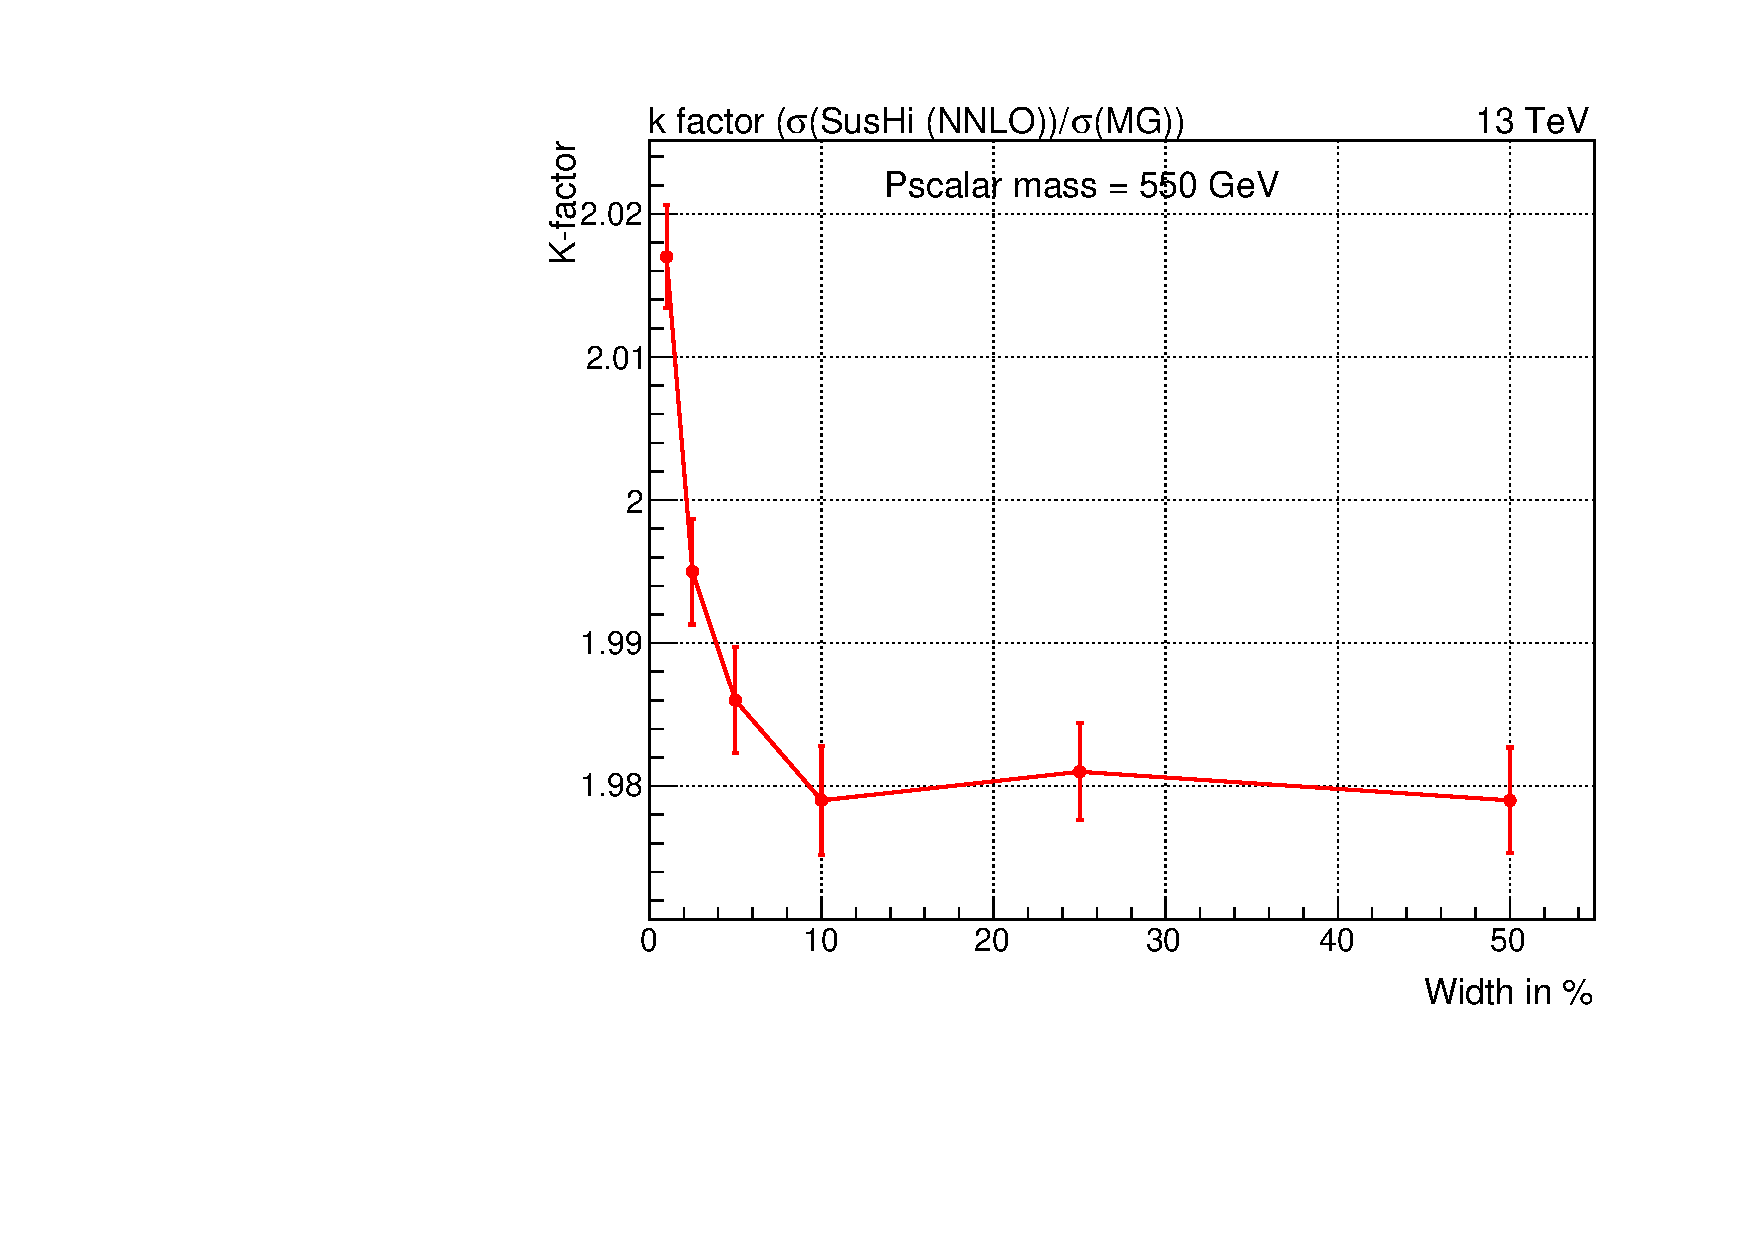
\includegraphics[scale=0.4]{fig/chapt4/k_factor_PScalar_m550_res.pdf}
& \hspace{-0.95cm} 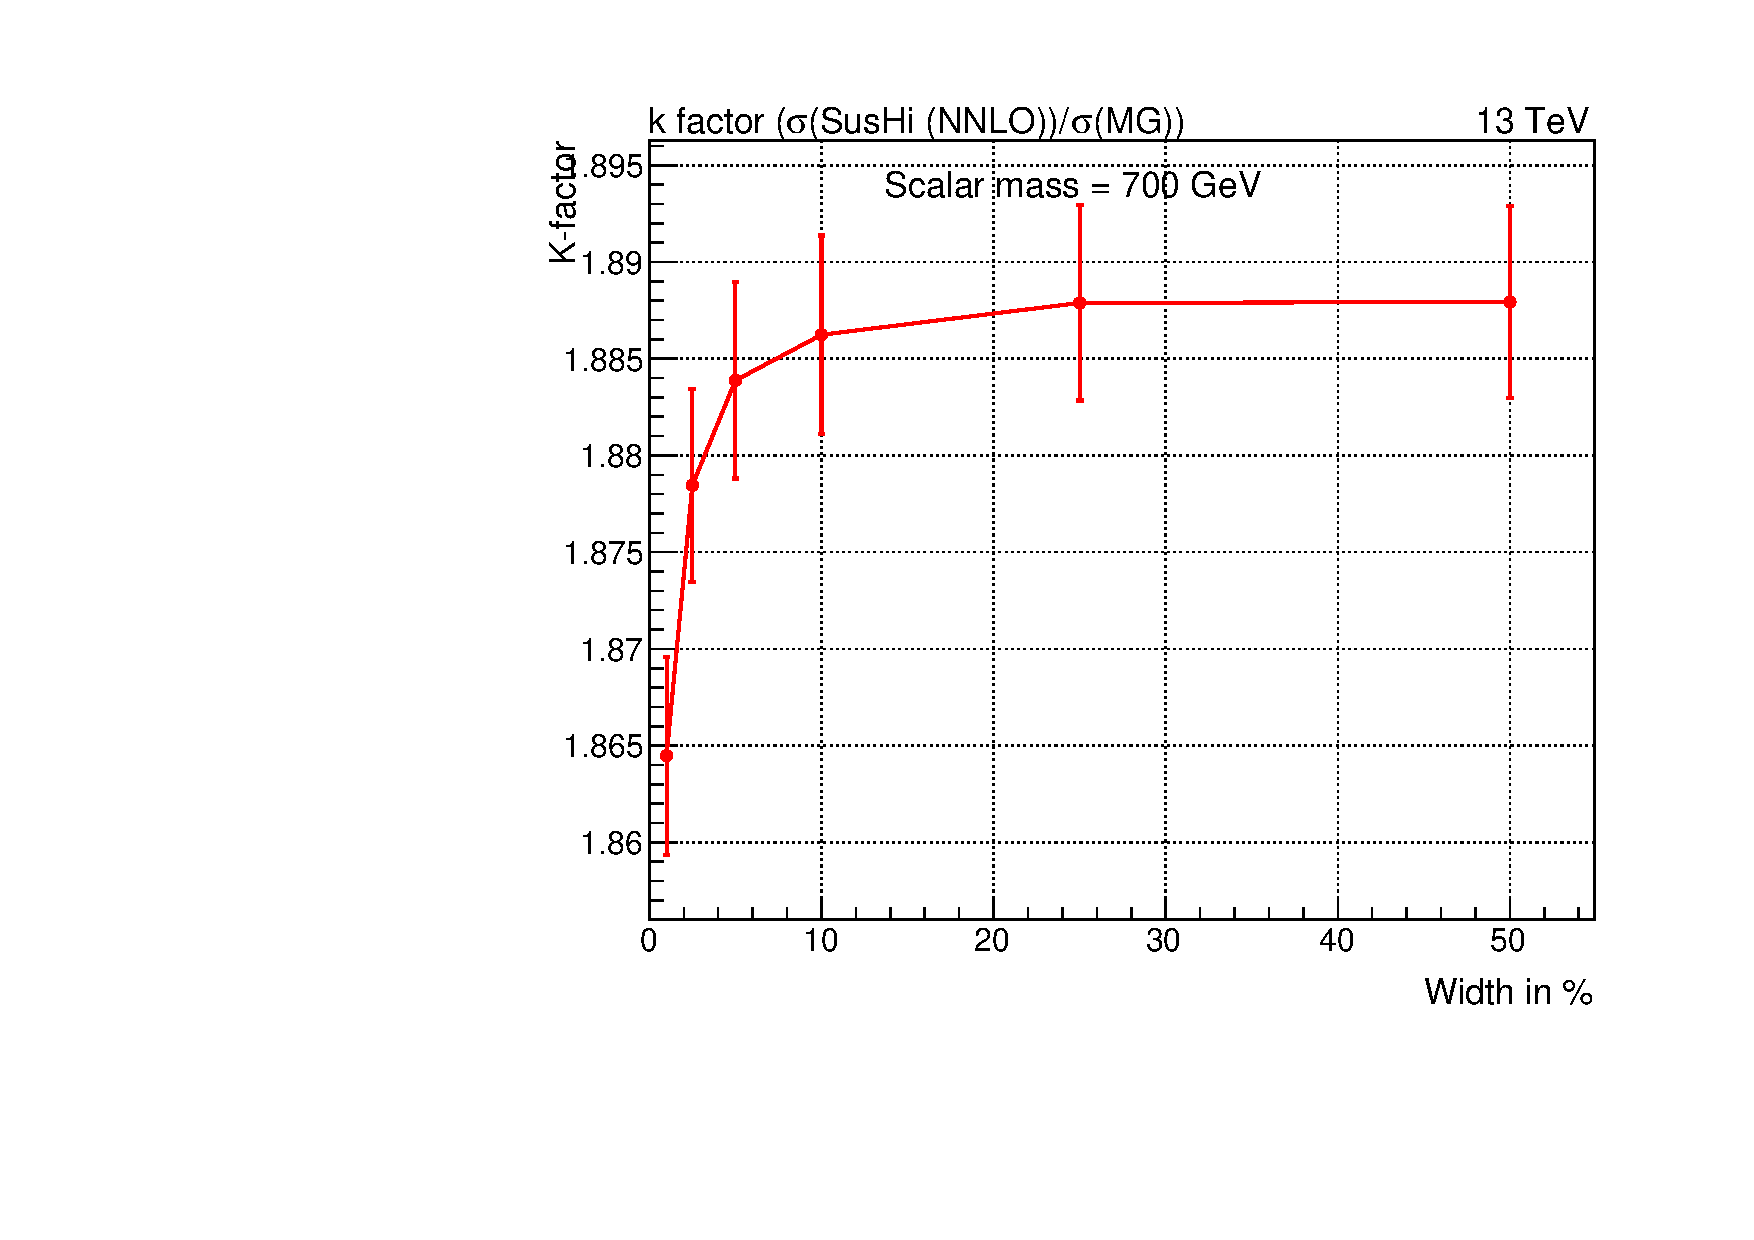
\includegraphics[scale=0.4]{fig/chapt4/k_factor_Scalar_m700_res.pdf}\\
($\mathbf{a}$)\qquad\qquad&($\mathbf{b}$)\qquad\qquad\\ \\
\caption{K-factor for pseudo-scalar mass = 550 GeV (a) and scalar mass = 700 GeV (b), obtained from the ratio of $\sigma_{NNLO}$(SusHi) to $\sigma$(MG). Both SusHi and MG LO cros sections are comparable which gives the same results if we use $\sigma_{LO}$(SusHi) instead of $\sigma_{LO}$(SusHi). For whole range of width, the k-factor shows univesitality which is easy to apply for other values of widths \label{fig:k_factor}.}
\end{tabular}
\end{figure}

\subsection{Top++}\label{subsec:top_pp}
The program Top++ \cite{Czakon:top_pp} calculates the total inclusive cross-section for top pairs production in hadronic collisions using two different approaches a) fixed order with NNLO accuracy and b) including soft-gluon resummation in Mellin space with full next-to-next-to-leading logarithmic order (NNLL) accuracy matched through NNLO. Top++ is the only publicly available program using soft-gluon resummation method for the $t\bar{t}$ inclusive production cross section in hadron colliders.
The program Top++ based on C++ coding in a modular and easy way with a single configuration file ($\texttt{top++.cfg}$) for user interface. The configuration file consists of simple input parameters like, type of collider, pdf set, pure fixed order calculation versus one with resummation, mass of top quark, LO, NLO and NNLO orders. For this work we use top++ to calculate the $t\bar{t}$ hadronic cross section upto NNLO accuracy with soft-gluon resummation and LO cross section without soft-gluon resummation. From these two cross sections, k-factor ($\sigma(NNLO)/\sigma(LO)$) has been calculated for further the scaling of interference. The input parameters used for this study;  


\section{Signal Modelling}\label{sec:signal}
\subsection{Signal Generation and Validation}

    




\clearpage{\pagestyle{empty}\cleardoublepage}
